\documentclass[tikz,border=10pt]{standalone}
\usepackage{tikz}

\begin{document}

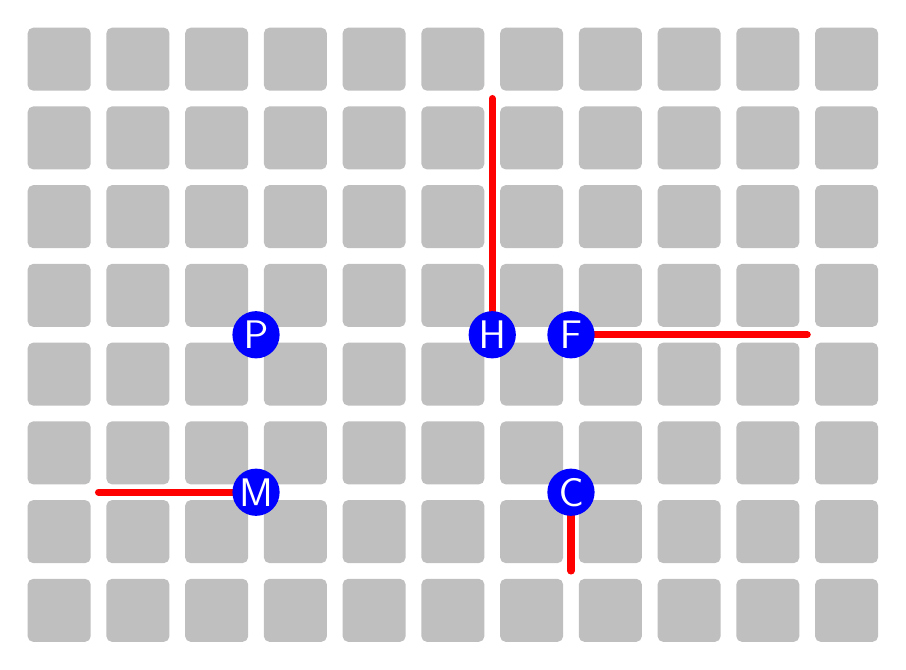
\begin{tikzpicture}[yscale=-1]

\def\height{8}
\def\width{11}

% Draw the grid
\foreach \x in {0,...,\numexpr\width-1\relax} {
    \foreach \y in {0,...,\numexpr\height-1\relax} {
        \fill[fill=gray!50, rounded corners=2pt] 
            (\x+0.1, \y+0.1) 
            rectangle ++(0.8, 0.8);
    }
}

% Highlighted red lines
\draw[red, line width=0.9mm, line cap=round] (1, 6) -- (3, 6); % Horizontal line
\draw[red, line width=0.9mm, line cap=round] (7, 4) -- (10, 4); % Horizontal line
\draw[red, line width=0.9mm, line cap=round] (7, 6) -- (7, 7); % Vertical line
\draw[red, line width=0.9mm, line cap=round] (6, 1) -- (6, 4); % Vertical line

% Labeled circles with text
\fill[blue] (7, 6) circle (0.3) node[white] {\Large{\textsf{C}}};
\fill[blue] (3, 4) circle (0.3) node[white] {\Large{\textsf{P}}};
\fill[blue] (6, 4) circle (0.3) node[white] {\Large{\textsf{H}}};
\fill[blue] (7, 4) circle (0.3) node[white] {\Large{\textsf{F}}};
\fill[blue] (3, 6) circle (0.3) node[white] {\Large{\textsf{M}}};

\end{tikzpicture}

\end{document}

